\subsubsection{Collection de matrices creuses de l'université de Floride}
La généralisation de l'approche proposée dans Taggre aux problèmes représentés par les 13 nains de Barkeley n'étant pas facile à montrer d'un point de vue théorique, nous nous sommes intéressés à l'utilisation de Taggre sur des exemples de problèmes correspondant à des graphes de tâches très variés.
%
La collection de matrices creuses de l'université de Floride est un ensemble de matrices provenant de diverses simulations.
%
Parmi toutes ces matrices, nous en avons choisi quatre ayant des motifs différents de ceux que nous pouvons retrouver en simulation de réservoir.
%
Nous ne nous intéressons pas aux propriétés physiques de ces simulations, mais seulement aux connexions des noeuds dans le graphe.
%
C'est pourquoi nous allons choisir des paramètres de simulation arbitraires pour le poids des tâches et pour les effets de cache.
%
Ces paramètres auront une incidence sur le choix des opérateurs d'agrégations.
%
Nous testerons ces différents opérateurs grâce à notre simulateur.


\begin{figure}[!h]
     \begin{center}
        \subfigure[Pajek/EPA]{
          \label{fig:florida_epa}
          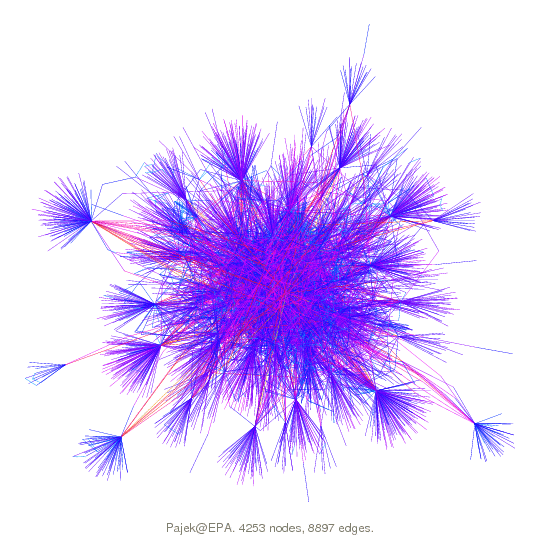
\includegraphics[width=0.45\textwidth]{florida_epa}
        } %
        ~
        \subfigure[SNAP/roadNet-PA]{
          \label{fig:florida_roadNet}
          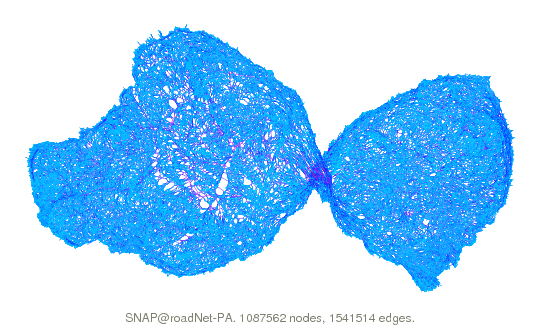
\includegraphics[width=0.45\textwidth]{florida_roadNet}
        }
        \subfigure[Gleich/wb-cs-stanford]{
          \label{fig:florida_wbcs}
          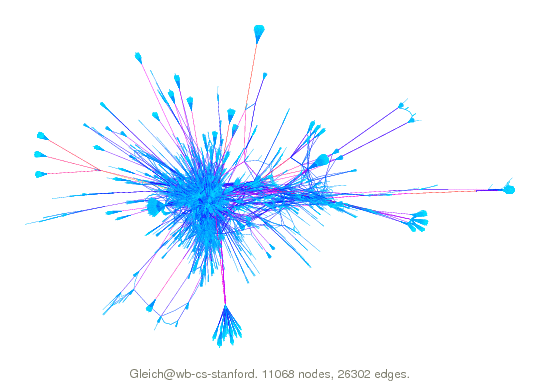
\includegraphics[width=0.45\textwidth]{florida_wbcs}
        }
        ~
        \subfigure[Williams/webbase-1M]{
          \label{fig:florida_webbase}
          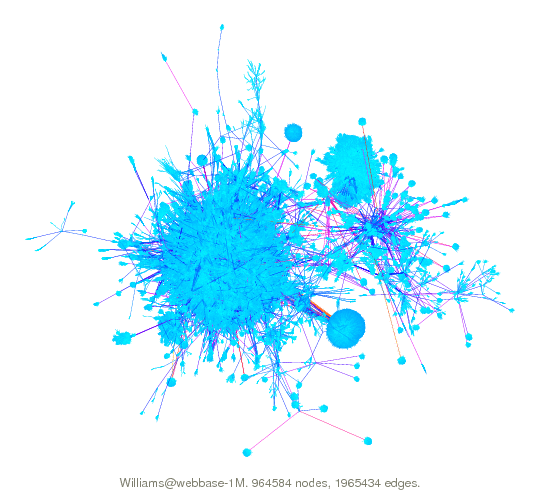
\includegraphics[width=0.45\textwidth]{florida_webbase}
        }
    \end{center}
    \caption{Représentation du graphe de connexions des quatre matrices choisies.}
    \label{fig:florida}
\end{figure}

%   (-_-)   %
\begin{table}[h!]
\begin{center}
  \begin{tabular}{|r|c|c|c|c|}
    \hline
    Nom de la & Nombre de       & Nombre de & Paramètre des   & Paramètre de\\
    matrice   & lignes/colonnes & non-zéros & effets de cache & granularité \\
    \hline
    Pajek/EPA             & 4~772     & 8~965     & 0,95 & 0,02  \\
    SNAP/roadNet-PA       & 1~090~920 & 3~083~796 & 0,70 & 1     \\
    Gleich/wb-cs-stanford & 9~914     & 36~854    & 0,50 & 0,001 \\
    Williams/webbase-1M   & 1~000~005 & 3~105~536 & 0,98 & 0,5   \\
    \hline
  \end{tabular}
  \captionof{table}{Descriptions des matrices utilisées.}
  \label{tab:florida}
\end{center}
\end{table}


Les premiers résultats concernent la matrice Pajek/EPA, ce graphe représente les liens de pages vers {\em www.epa.gov}.
%
Le graphe est plutôt petit (environ 5000 noeuds), nous n'aurons donc pas beaucoup de tâches.
%
Nous avons choisi pour le simulateur de tâches des valeurs représentant des tâches plutôt grosses (50 fois le coût d'ordonnancement) et qui ne bénéficie presque pas des effets de cache.
%
L'agrégation ne permet qu'un gain de 30\% dans les meilleurs cas (Table~\ref{tab:epa}).
%
Aucun opérateur d'agrégation ne se démarque des autres.

%   (-_-)   %
\begin{table}[h!]
  \begin{center}
    \begin{tabular}{|c|c|c|c|c|c|c|c|c|c|c|}
      \hline
      \multicolumn{11}{|c|}{Types d'agrégations}\\
      \O & D(2) & D(4) & D(8) & D(16) & D(32) & F(24) & F(36) & F(42) & F(64) & C \\
      \hline
      598 & 403 & 400 & 428 & 435 & 523 & 407 & 392 & 392 & 392 & 406 \\
      \hline
    \end{tabular}
    \caption{Résultats du simulateur d'exécution de tâches sur Pajek/EPA sur 12 coeurs de calculs.}
    \label{tab:epa}
  \end{center}
\end{table}


Les résultats suivants concernent un graphe représentant les intersections de routes de Pennsylvanie (SNAP/roadNet-PA).
%
Le graphe est assez grand, nous pourrons agréger des noeuds ensemble.
%
La granularité des tâches que nous avons choisie est petite, l'ordonnanceur met autant de temps à ordonnancer la tâche que la tâche met à s'exécuter.
%
De plus, les effets de cache peuvent améliorer le temps de calcul.
%
L'opérateur D se démarque des autres opérateurs en divisant par deux le temps de calcul (Table~\ref{tab:roadnet}).
%
L'opérateur F n'a pas fourni une bonne agrégation à cause des effets de cache.


%   (-_-)   %
\begin{table}[h!]
\begin{center}
  \begin{tabular}{|c|c|c|c|c|c|c|c|c|c|c|}
    \hline
    \multicolumn{11}{|c|}{Types d'agrégations}\\
    \O & D(16) & D(64) & D(256) & D(1500) & D(2048) & F(24) & F(36) & F(42) & F(64) & C \\
    \hline
    136370 & 84244 & 75919 & 72145 & 69359 & 69607 & 92211 & 80529 & 80179 & 80190 & 181826 \\
    \hline
  \end{tabular}
  \caption{Résultats du simulateur d'exécution de tâches sur SNAP/roadNet-PA sur 12 coeurs de calculs.}
  \label{tab:roadnet}
\end{center}
\end{table}


Le troisième cas test représente les liens entre les pages du site web de stanford (Gleich/wb-cs-stanford).
%
Il s'agit d'un petit graphe d'environ 10000 noeuds.
%
Les tâches ont une granularité grossière et peuvent bénéficier d'améliorations des effets de cache.
%
Tous les opérateurs d'agrégations donnent environ les mêmes résultats (Table.~\ref{tab:stanford}).


%   (-_-)   %
\begin{center}
  \begin{tabular}{|c|c|c|c|c|c|c|c|c|c|c|}
    \hline
    \multicolumn{11}{|c|}{Types d'agrégations}\\
    \O & D(2) & D(4) & D(8) & D(16) & D(32) & F(24) & F(36) & F(42) & F(64) & C \\
    \hline
    1267 & 765 & 729 & 733 & 753 & 923 & 739 & 736 & 736 & 737 & 722 \\
    \hline
  \end{tabular}
  \captionof{table}{Résultats du simulateur d'exécution de tâches sur Gleich/wb-cs-stanford sur 12 coeurs de calculs.}
  \label{tab:stanford}
\end{center}


Le dernier cas test est une matrice de connexions de site web (Williams/webbase-1M).
%
La matrice est grande, nous avons choisi comme paramètre de tâche, une granularité fine avec un très petit gain sur les effets de cache.
%
Les gains liés à l'agrégation sont faibles (35\%) et les opérateurs D et F donnent les mêmes performances.
%
L'opérateur C n'a pas été très utile.


%   (-_-)   %
\begin{center}
  \begin{tabular}{|c|c|c|c|c|c|c|c|c|c|c|}
    \hline
    \multicolumn{11}{|c|}{Types d'agrégations}\\
    \O & D(16) & D(64) & D(256) & D(1500) & D(2048) & F(24) & F(36) & F(42) & F(64) & C \\
    \hline
    125512 & 84898 & 82837 & 82913 & 86024 & 88551 & 82453 & 82490 & 89461 & 87427 & 124889 \\
    \hline
  \end{tabular}
  \captionof{table}{Résultats du simulateur d'exécution de tâches sur Williams/webbase-1M sur 12 coeurs de calculs.}
  \label{tab:webbase}
\end{center}

